\chapter{Euler Equations}

\section{General formulations}
The Euler equations in the conservative form can be stated using the Einstein summations as
\begin{align}
	\pdv{\rho}{t} + \pdv{}{x_j}\left(\rho u_j\right) &= 0\\
	\pdv{}{t} \left( \rho u_i \right) + \pdv{}{x_j} \left(\rho u_i u_j + p \delta_{ij} \right) &= 0\\
	\pdv{}{t} \left( \rho E \right) + \pdv{}{x_j} \left[(\rho E + p) u_j \right] &= 0
\end{align}
those are the continuum equation, momentum equation and energy equation.
They are close using the ideal gas equation
\begin{equation}
	p = \rho R T
\end{equation}
and the equation for internal energy
\begin{equation}
	\rho E = \frac{\gamma}{\gamma - 1} p + \frac{1}{2} \rho |u|^2.
\end{equation}

It can also be written in vector form as
\begin{align}
\pdv{\rho}{t} + \nabla \cdot (\rho \bb{u}) = 0\\
\pdv{(\rho \bb{u})}{t} + \nabla \cdot (\rho \bb{u} \bb{u}^T) + \nabla p - \bb{f} = 0\\
\pdv{E}{t} + \nabla \cdot (\bb{u}(E + p)) = 0
\end{align}
where
\begin{equation}
	E = \rho e + \frac{1}{2} \rho \|\bb{u}\|^2
\end{equation}
and
\begin{equation}
	e = T c_v.
\end{equation}

According to Anderson, JR. 6th edition:
Conservation of mass (continuity equation)
\begin{equation}
	\pdv{\rho}{t} + \nabla \cdot (\rho \bb{u}) = 0
\end{equation}
Momentum equation
\begin{align}	
	\pdv{(\rho u)}{t} + \nabla \cdot (\rho u \bb{u}) &= - \pdv{p}{x} + \rho f_x + (F_x)_{\mm{viscous}}\\
	\pdv{(\rho v)}{t} + \nabla \cdot (\rho v \bb{u}) &= - \pdv{p}{y} + \rho f_y + (F_y)_{\mm{viscous}}\\
	\pdv{(\rho w)}{t} + \nabla \cdot (\rho w \bb{u}) &= - \pdv{p}{z} + \rho f_z + (F_z)_{\mm{viscous}}
\end{align}
where $f$ are body forces like gravitation and electromagnetic and $F$ are forces due to viscosity.
The energy equation
\begin{multline}
	\pdv{}{t}\left[\rho \left(e + \frac{1}{2}\|\bb{u}\|^2 \right) \right] + \nabla \cdot \left[\rho \left(e + \frac{1}{2}\|\bb{u}\|^2 \right) \bb{u} \right] = \\
	\rho \dot{q} - \nabla \cdot(p \bb{u}) + \rho(\bb{f} \cdot \bb{u}) + \dot{Q}_{\mm{viscous}} + \dot{w}_{\mm{viscous}}
\end{multline}
where $\dot{Q}_{\mm{viscous}}$ and $\dot{w}_{\mm{viscous}}$ are the viscous heat and work respectively.
Here again we have 
\begin{equation}
	e = T c_v
\end{equation}
which is equivalent for noble gases to
\begin{equation}
	e = \frac{3}{2} \frac{k_B}{m} T
\end{equation}
where $m$ is the per molecule mass.

\section{Inviscid steady state form}
Disregarding body forces in vector form
\begin{align}
	\nabla \cdot (\rho \bb{u}) = 0\\
	\nabla \cdot (\rho \bb{u} \bb{u}^T) + \nabla p = 0\\
	\nabla \cdot (\bb{u}(E + p)) = 0
\end{align}
or in the Einstein notation
\begin{align}
	\pdv{\rho u_j}{x_j} = 0\\
	\pdv{}{x_j} \left(\rho u_i u_j + p \delta_{ij} \right) = 0\\
	\pdv{}{x_j} \left[(E + p) u_j \right] = 0
\end{align}
again with
\begin{align}
	E &= \rho e + \frac{1}{2} \rho \| \bb{u} \|^2\\
	e &= c_v T\\
	e &= \frac{3}{2} k_B T.
\end{align}

\section{Discritization}
Using finite difference methods with non--equidistant spacing as seen in Fig.~\ref{fig:non-equidistant_spacing}.
%---------------------------------------------------------------------------------------------------------------
\begin{figure}[H]
	\centering
	\includegraphics[width=0.7\textwidth]{figures/DM_non_equidistant.png}
	\caption{Non--equidistant spacing on a regular grid.}
	\label{fig:non-equidistant_spacing}
\end{figure}
%---------------------------------------------------------------------------------------------------------------
Forward differential coefficient and backward differential coefficient
\begin{align}
	\pdv{y}{x} = \frac{y(x_{i+1}) - y(x_{i})}{x_{i+1} - x_{i}}\\
	\pdv{y}{x} = \frac{y(x_{i}) - y(x_{i - 1})}{x_{i} - x_{i - i}}
\end{align}
using Taylor expansion
\begin{equation}
	Ty(x;a) = y(a) + \left.\pdv{y}{x}\right|_{x = a}(x - a)
\end{equation}
we get
\begin{align}
	y(x_{i+1}) = y(x_i) + \left.\pdv{y}{x}\right|_{x = x_i}(x_{i+1} - x_i)\\
	y(x_{i-1}) = y(x_i) + \left.\pdv{y}{x}\right|_{x = x_i}(x_{i-1} - x_i)
\end{align}
we get
\begin{align}
	y(x_{i+1}) - y(x_{i-1}) = y'(x_i)(x_{i+1} - x_i) - y'(x_i)(x_{i-1} - x_i)\\
	y(x_{i+1}) - y(x_{i-1}) = y'(x_i)(x_{i+1} - x_{i-1})
\end{align}
and therefore
\begin{align}
	\frac{y(x_{i+1}) - y(x_{i-1})}{x_{i+1} - x_{i-1}} = y'(x_i).
\end{align}
For second order we have
\begin{align}
	y''(x_i) = \frac{\frac{y(x_{i+1}) - y(x_i)}{x_{i+1} - x_i} - \frac{y(x_i) - y(x_{i-1})}{x_i - x_{i-1}}}{x_{i+1} - x_{i}}
\end{align}
using the definitions
\begin{align}
	\Delta x^+ &= x_{i+1} - x_i\\
	\Delta x^- &= x_{i} - x_{i-1}\\
	\Delta \overline{x} &= \Delta x^+ - \Delta x^-
\end{align}
and therefore
\begin{align}
	y''(x_i) &= \frac{y(x_{i+1}) - y(x_i)}{\Delta x^+\Delta x^+} - \frac{y(x_i) - y(x_{i-1})}{\Delta x^- \Delta x^+}\\
	y''(x_i) &= \frac{\Delta x^- y(x_{i+1}) - \Delta x^-y(x_i) - \Delta x^+ y(x_i) + \Delta x^+ y(x_{i-1})}{\Delta x^+ \Delta x^- \Delta x^+}\\
	y''(x_i) &= \frac{\Delta x^-\,y(x_{i+1}) - \Delta \overline{x}\,y(x_i) + \Delta x^+\,y(x_{i-1})}{\Delta x^+\,\Delta x^-\,\Delta x^+}.
\end{align}
For second order, second derivative we have
\begin{align}
	y''(x_i) = \frac{\frac{y(x_{i+2}) - y(x_i)}{x_{i+2} - x_i} - \frac{y(x_{i}) - y(x_{i-2})}{x_{i} - x_{i-2}}}{x_{i+1} - x_{i-1}}.
\end{align}